\documentclass[a4paper, 12pt]{article}
\usepackage{cmap}
\usepackage[utf8]{inputenc}
\usepackage[english, russian]{babel}
\usepackage[left=2cm, right=2cm, top=2cm, bottom=2cm]{geometry}
\usepackage{amsfonts,amssymb}
\usepackage{amsmath}
\usepackage{amsthm}
\usepackage{titlesec}
\usepackage{graphicx}
\usepackage{mathtools}
\usepackage{hyperref}

 \newcommand{\tit}[1]{\begin{center}{\bf{\Large #1}}\end{center}}
 \newcommand{\aut}[1]{\centerline{{\bf #1}}}
 \newcommand{\cityorg}[1]{\centerline{\it #1}}
 \newcommand{\email}[1]{\centerline{{\small e-mail: #1}}\vspace{\baselineskip}}
\providecommand{\keywords}[1]{\textbf{\textit{Ключевые слова:}} #1}
\newcommand{\norm}[1]{\left\lVert#1\right\rVert}
\newcommand{\normb}[1]{\left\lVert\textbf{#1}\right\rVert}

\begin{document}

\sloppy
 \tit{Цилиндрическая маскировка при помощи оптимизированных конечных многослойных параметров для наклонного падения}
 \aut{Baile Zhang and Bae-Ian Wu}

\begin{abstract}
Мы предлагаем многослойную цилиндрическую маскировочную оболочку, оптимизированную для непрямого падения путем комбинации аналитического формализма и применении генетических алгоритмов. 
Мы покажем, что используя только четыре однороных, анизотропных слоя с параметрами, не принимающими больших значений, рассеяние для падения под непрямым углом может быть уменьшено на 
два порядка. Несмотря на то, что оптимизация применялась для одного угла падения, оболочка показывает уменьшение рассеяния для широкого диапазона углов.
\end{abstract}

В последнее время было приложено много усилий для проектирования и воплощения метаматериальных 
маскирующих оболочек используя трансформационные методы. 

% \begin{figure}[t]
%   \centering
%   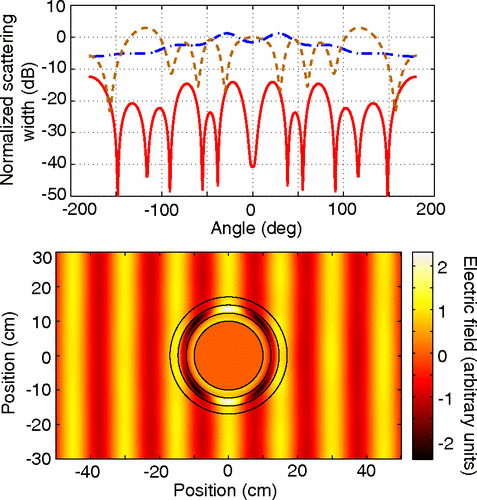
\includegraphics[height=0.4\paperheight, width=0.55\paperwidth]{fig4.png}
%   \caption{}
%   \label{fig:4}
% \end{figure}

\end{document}
